
\chapter{Mathematical Formulation}

\section{Kinematics}
Consider a certain particle, initially located at the coordinate $\X$. During deformation, this particle follows a path 
\begin{gather}
\x = \x(\X,t).
\end{gather}
Let $\u(\X, t)$ be the displacement of the material particle located at $\X$. Then
\begin{gather}
     \u(\X, t) = \x(\X, t) - \X.
\end{gather}
The total deformation gradient and Green-Lagrange strain are denoted by $\F$ and $\E$, respectively. Therefore, 
\begin{align}
    \F &= \pdiff{\x}{\X} = \nablaX \u + \I, \\
    \E &= \fc{1}{2}(\F^\T \cdot \F - \I)
\end{align}
where $\I$ is the second-order isotropic tensor.

Let $\{\hat{\bm{e}}_1, \hat{\bm{e}}_2, \hat{\bm{e}}_3\}$ be the orthonormal basis in the reference configuration. corresponding components of $\X$ are denoted by $X$, $Y$ and $Z$ and that of $\u$ by $u$, $v$ and $w$. In the present study, plane strain deformation is assumed. Therefore, the components of F are given by \citep{2009ContMechLai} 
\begin{align}
[\F] = 
\begin{bmatrix}
    1 + \pdiff{u}{X} && \pdiff{u}{Y} && 0 \\
    \pdiff{v}{X} && 1 + \pdiff{v}{Y} && 0 \\
    0 && 0 && 1
\end{bmatrix} = \tensor{F}. \label{eq:F_tensor}
\end{align}
Both Inelastic and elastic deformation gradients are considered to be finite \citep{2011JMPSBower}. Hence, a multiplicative decomposition of $\F$ into elastic and inelastic deformation is necessary. As shown in \ref{fig:decomposition}, the body is first considered to reach an intermediate stress-free state, and then it undergoes an elastic deformation to reach the current configuration. As derived by \citet{1969Lee}, the total deformation gradient   
\begin{gather}
\F = \F^{\el} \cdot  \F^{\inel} \label{eq:F_decomposition} \\
\text{where, } \F^{\el} = \pdiff{\x}{\x_I} \text{ and } \F^{\inel} = \pdiff{\x_{I}}{\X} \nonumber
\end{gather}
\begin{figure}[H]
    \centering
    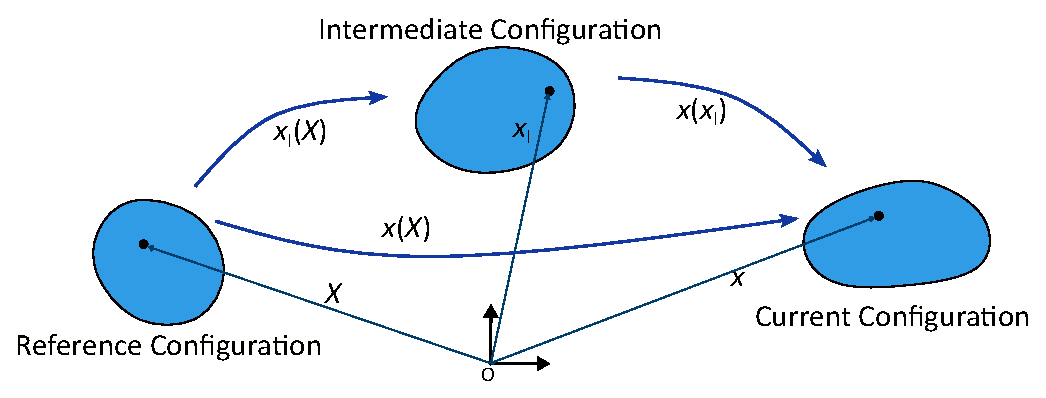
\includegraphics[width=\textwidth]{figures/mathFormFigs/decomposition.eps}
    \caption{Decomposition of the deformation gradient into the elastic and inelastic part.}
    \label{fig:decomposition}
\end{figure}
$\F^{\el}$ and $\F^{\inel}$ denote the deformation gradients due to elastic deformation and inelastic deformation, respectively.

The inelastic deformation gradient tensor, $\F^{\inel}$, has contributions from two sources. It is further decomposed as 
\begin{gather}
    \F^\inel = \F^\c \cdot \F^\p. \label{eq:Finel_decomposition}
\end{gather}
Where $\F^\c$ and $\F^\p$ are deformation gradients due to diffusion and plastic flow, respectively.

\section{Viscoplastic Flow}
A viscoplastic constitutive relation of the following form is considered:
\begin{gather}
\DP = \pdiff{G(\sigmaeff)}{\DCS}
\end{gather}
Where $\DP$ is the rate dependent plastic deformation tensor, $G(\sigmaeff)$ is the flow potential, $\DCS$ is the deviatoric part of Cauchy stress tensor and $\sigmaf$ is yield strength defined as 
\[ \sigmaf =  \begin{cases} 
    \sigma_{f, \si} & \text{ for Silicon} \, \, (-L/2 \le X \le L/2 {\rm{ \quad and \quad}} 0 \le Y \le H) \\
     \sigma_{f, {\rm{SEI}}} & \text{ for SEI layer} \, \, (-L/2 \le X \le L/2 {\rm{ \quad and \quad}} 0 \le Y \le H+H_{\rm{SEI}})
\end{cases}
\]

Various studies \citep{2011JMPSBower,2012JMPSCui} have adopted a power law of the following form for flow potential
\begin{align}
G(\sigmaeff) &= \fc{\sigmaf \dZEROdot}{\mathrm{m}+1}\left(\fc{\sigmaeff}{\sigmaf}-1\right)^{\mathrm{m}+1}\heavi \\
\Rightarrow \mathbf{D}^{\rm{P}} &= \fc{3 \DCS \dZEROdot}{2 \sigmaeff}\left(\fc{\sigmaeff}{\sigmaf}-1\right)^{\mathrm{m}}\heavi.
\end{align}
where $\sigmaeff$ is the effective von Mises stress, defined in section \ref{section:MechEqbm}, H is the unit step function, $\sigmaf$ is the yield strength of Silicon, m is the stress exponent for plastic flow and $\dZEROdot$ is the strain rate for plastic flow. Considering an irrotational plastic flow \citep{2005JMPSGurtin, 2005IJPGurtin,2023IJSSAmit} 
\begin{align}
{\color{red}\mathbf{D}^{\rm{P}}} &= \F^{\el} \cdot \F^{\rm{c}} \cdot \dot{\F}^\p \cdot \inv{\F^\p} \cdot \inv{\F^{\rm{c}}} \cdot \inv{\F^{\el}}  \\
\Rightarrow \dot{\F}^\p &= \inv{J} \fc{3}{2} \fc{\Mel \cdot \F^\p}{\sigmaeff} \dZEROdot \left( \fc{\sigmaeff}{\sigmaf} - 1 \right)^\m \heavi  \\
\text{where }\Mel &= J (\F^\el)^\T \cdot \DCS \cdot (\F^\el)^\mT \label{eq:M_tensor} \\
\text{and} J &= \mathrm{det}(\F). 
\end{align}
$\Mel$ is the deviatoric part of Mandel stress \citep{1971Mandel}. The expression for Mandel stress is 
\begin{nonumbereq}
\mathbf{M}^{\el} = J (\F^{\el})^{\T} \CS \invT{F^{\el}}.
\end{nonumbereq}
Attributing to the assumption of plane strain, $\F^{\rm{p}}$ is considered to be of the following form:
\begin{gather}
 [\F^\p] = \tensor{\lambda}.
\end{gather}
Since, det($\F^\p$) = 1
\begin{gather}
\lamzz = 1/(\lamxx \lamyy - \lamxy \lamyx).
\end{gather}



\section{Diffusion Induced Deformation}
The compound formed between Lithium and Silicon is of the form $\text{Li}_{\chi}$Si. Let the stoichiometric concentration and maximum concentration of Lithium ions per atom of Silicon be denoted by $\chi_0$ and $\chi_{\rm{max}}$. Defining a non-dimensional measure of the Li-ions concentration as $\tc = (\chi-\chi_{0})/\xmax$. Since $\chi_{0}$ is the stoichiometric ratio, it signifies the stress-free state of the particle, and hence, $\tc$ is a measure of the deviation of the particle from the undeformed state. The deformation due to lithiation is quantified by an isotropic deformation gradient denoted by $\F^\c$ and given by
\begin{gather}
\F^\c = (\jc)^{1/3} \I
\end{gather}
where \begin{nonumbereq}\jc = 1 + 3 \eta \xmax \tc\end{nonumbereq} is the volumetric change experienced by the Silicon film upon insertion of Li-ions. $\eta$ is a material parameter giving the rate of change in volume w.r.t. $\tc$. It may be noted that as $\tc$ approaches 1, $\mathrm{det}(\F^\c)$ approaches 4. Therefore, the body undergoes a volumetric change of about 300\% due to the diffusion of Li-ions, justifying the use of large deformation analysis.

Since SEI is permeable to lithiation, $\F^\c$ will be considered only for Silicon. Therefore, for the purpose of modelling, $\tc$ is considered zero in SEI, making $\F^\c$ equal to $\I$.
\section{Mechanical Equilibrium } \label{section:MechEqbm}
From equations \ref{eq:F_decomposition} and \ref{eq:Finel_decomposition},
\begin{align}
\F^{\el} &=  \F \cdot \inv{\F^{\p} \cdot \F^{\c}}. \label{eq:Fel_tensor}
\end{align}
The elastic Green-Lagrange strain
\begin{nonumbereq}
\E^{\el} = \fc{1}{2} \left[ (\F^\el)^\T \cdot  \F^\el - \I \right].
\end{nonumbereq}

The constitutive relation for the elastic deformation is expressed in terms of the strain energy per unit volume in the intermediate configuration, $\hat{w}(\F, \tc)$. Denoting the elasticity tensor of Silicon by $\mathbb{C}$ and its components by $C_{ijkl}$,
\begin{gather}
\hat{w}(\F, \tc) = \fc{1}{2} C_{ijkl} \Eel{ij} \Eel{kl}.
\end{gather}
$\mathbb{C}$ is concentration-dependent and assumed to be isotropic. Hence, its components can be expressed in terms of Lam\'{e} coefficients as 
\begin{align}
 C_{ijkl}(\tc) &= \lambda_{\rm{mat}}(\tc)\delta_{ij} \delta_{kl} +  \mu_{\rm{mat}}(\tc)(\delta_{ik} \delta_{jl} + \delta_{il} \delta_{jk}). \\
\implies \hat{w}(\F, \tc) &= \left[\lamSic (\tr{\E^\el})^2 + 2 \muSic \E^{\el}:\E^{\el}\right].
\end{align}
The lam\'{e} parameters, $\lamSic$ and $\muSic$ are given by
\begin{align}
\lamSic = \fc{\EMatc \nuMat}{(1+\nuMat)(1-2\nuMat)},
&& \muSic = \fc{\EMatc}{2(1+\nuMat)}. \nonumber
\end{align}
The material properties $\EMatc$ and $\nuMat$ are defined domainwise as follows:
\[\EMatc = \begin{cases}
 E_{\text{si}}(1 + \eta_{\rm{E}} \chi_{\rm{max}} \tc) \text{\quad for Silicon} \\
 E_{\rm{SEI}} \text{\quad for SEI }
\end{cases} \text{ and }
\nuMat = \begin{cases}
\nu_{\si} \text{\quad for Silicon} \\
\nu_{\rm{SEI}} \text{\quad for SEI }
\end{cases}\]
The elastic second Piola-Kirchhoff stress is denoted by $\PKS^\el$. Therefore, 
\begin{align}
\PKS^\el &= \pdiff{\hat{w}(\F, \tc)}{\E^{\el}}\nonumber \\
\implies  \PKS^\el &= \lamSic \tr{\E^\el}\I + 2 \muSic \E^\el. \label{eq:Sel_tensor}
\end{align}
Let $\PKS$ denote the second Piola-Kirchhoff stress. Now, by pulling back $\PKS^{\el}$ from the intermediate configuration to the reference configuration \citep{2010Gurtin} the second Piola-Kirchhoff stress is obtained as
\begin{align}
    \PKS = J^{\inel} \, \inv{\F^\inel} \cdot  \PKS^\el \cdot  \invT{\F^\inel} &= \jc \, \inv{\F^{\p} \cdot \F^{\c}} \cdot \PKS^{\el} \cdot \invT{\F^\p \cdot \F^\c}\nonumber\\
\implies \PKS &= (\jc)^{1/3} \inv{\F^\p} \cdot \PKS^{\el} \cdot  \invT{\F^\p}.\label{eq:S_tensor}
\end{align}
The first Piola-Kirchhoff stress is
\begin{gather}
\PK = \F \cdot  \PKS  \label{eq:P_tensor}.
\end{gather}
The Cauchy stress tensor, $\CS$, is given by 
\begin{nonumbereq}\CS = \inv{J} \F \cdot  \PKS  \cdot  \F^\T.
\end{nonumbereq} The deviatoric part of Cauchy stress is \begin{nonumbereq}\DCS = \CS - (1/3)\tr{\CS}\I.
\end{nonumbereq}
The von Mises stress is 
\begin{nonumbereq}
\sigmaeff = \sqrt{\fc{3}{2}\tau_{ij}\tau_{ij}}. 
\end{nonumbereq}

In the absence of any body forces, the conservation of momentum leads to 
\begin{gather}
\bm{\nabla}_\X \cdot \PK = 0.
\end{gather}

\section{Diffusion}
Assuming flux to be negligible in the $z$ direction, the conservation of mass is given by
\begin{gather}
\pdiff{c}{t} = - \bm{\nabla}_\X \cdot \bm{j} = -\left(\pdiff{j_X}{X} + \pdiff{j_Y}{Y}\right).
\end{gather}
Where $\bm{j}$ is the flux vector and $c$ is a dimensional measure of Li-ions concentration, defined as 
\begin{nonumbereq}
 c = \tc \, \xmax/\vmb.
\end{nonumbereq}
In the current configuration the flux is denoted by $\bm{\hat{j}}(\x, t)$ and it is given by: \note{cite a paper which describes the following equation}
\begin{gather}
 \bm{\hat{j}(\x, t)} = -\fc{1}{R_g T} \fc{D \xmax \tc}{\vmb} \nabla_{\x} \mu
\end{gather} 
where $R_g$ is the universal gas constant, $T$ is the operating temperature, $D$ is the diffusivity of Li$_{\chi}$Si, $\vmb$ is the partial molar volume of Silicon and $\mu$ is the chemical potential. Diffusivity is related to the state of stress by the following equation:
\begin{gather} 
 D = D_0 \rm{exp}(\fc{\alpha S_h}{E_0}) = D_0 \rm{exp}\left(\alpha \frac{{S}_{11}+{S}_{33}}{2 E_0}\right)
\end{gather}
where $E_0$ is defined in section \ref{section:nonDim}.\\
In the reference configuration, the flux is $\bm{j}(\X, t)=J\inv{\F} \cdot \bm{\hat{j}}$ \note{how is the previous expression derived}. Now, 
\begin{align}
 (\nabla_{\x} \mu)_{i} &= \pdiff{\mu}{x_i} \nonumber \\
 &= \pdiff{\mu}{X_j}\pdiff{X_j}{x_i} \nonumber\\
\implies \nabla_{\x} \mu &= \F^{-\T} \cdot \nabla_{X}\mu.
\end{align}
From above equations, the flux, $\bm{j}(\X, t)$, in Lagrangian description is expressed as
\begin{align}
\bm{j} = - \fc{1}{R_g T} \fc{D\xmax \tc}{V^b_m} \inv{\F} \cdot \invT{\F} \cdot \nablaX \mu.
\end{align}
The chemical potential $\mu$ is composed of two parts: $\mu = \mu_0 + \mu_{\rm{s}}$, where $\mu_0$ and $\mu_{\rm{s}}$ are the stress-independent and stress-dependent part, respectively. $\mu_0$ can be written as \begin{nonumbereq}
\mu_0 = R_g T \rm{log}(\gamma \tc), 
\end{nonumbereq} where $\gamma$ is the activity coefficient and considered to be concentration dependent, given by the following equation:
\begin{align}
 \gamma &= \fc{1}{1-\td{c}}\text{exp}(\fc{1}{R_g T}[2(A_0 - 2B_0)\td{c} - 3(A_0 - B_0)(\td{c}^2)]).
\end{align}
The stress-dependent part of the chemical potential is \citep{2012JMPSCui}
\begin{align}
\mu_s &= \fc{V_m^b}{\xmax}\left[-\fc{1}{3}\pdiff{\jc}{\tc}\tFel{im}\tFel{in}{C}_{mnkl}\tEel{kl} + \fc{1}{2}\left(\jc \pdiff{C_{ijkl}}{\tc} + \pdiff{\jc}{\tc} C_{ijkl}\right)\tEel{ij}\tEel{kl}\right].
\end{align}
State of charge is a measure of the degree of lithiation. It is expressed as an average concentration over the domain as follows:
\begin{align}
 \rm{soc} &= \fc{1}{LH}\int_{-L/2}^{L/2} \int_0^H \tc \rm{d}y \rm{d}x  \nonumber \\
&= H^2\fc{1}{LH} \int_{-L/2H}^{L/2H} \int_0^1 \tc(\td{x}, \td{y}) \rm{d}\td{y} \rm{d}\td{x} \nonumber \\
&= \fc{H}{L}\int_{-L/2H}^{L/2H} \int_0^1 \tc(\td{x}, \td{y}) \rm{d}\td{y} \rm{d}\td{x} 
\end{align}

\section{Non-dimensionalisation}\label{section:nonDim}
\begin{align}
 \td{j}_X, \td{j}_Y, \td{J}_0, \td{\bm{j}} &=  \fc{H \vmb}{(\xmax D_0)} (j_X, j_y, J_0, \bm{j}) \\
 \tX, \tY, \tu, \tv &= \fc{1}{H}(X, Y, u, v) \\
 \td{t} &= D_0 t/H^2 \\
\tmusi, \tlamsi, \td{E}_{\text{si}} &= \fc{1}{E_0} (\mu_{\text{si}}, \lambda_{\text{si}}, E_{\text{si}}) 
\text{,where }  E_0 = \fc{R_g T}{\vmb} \\
\td{\mu}_0, \td{\mu}_1, \td{\mu}_2, \td{\mu}_3 &= \fc{1}{R_g T}(\mu_0, \mu_1, \mu_2, \mu_3) \\
\td{D} &= \fc{D}{D_0} \\
\dot{\td{d}}_{0} &= \fc{\dZEROdot H^2}{D_0} \\
\td{\PKS}^{\el}, \td{\PKS}, \td{\PK}, \td{\CS}, \td{\DCS}, \td{\mathbf{M}}^{\el}_{0}, \td{\sigma}_{\rm{eff}}, \td{\sigma}_{\rm{f}} &= \fc{1}{E_0}(\PKS^{\el}, \PKS, \PK, \CS, \DCS, \mathbf{M}^{\el}_{0}, \sigmaeff, \sigmaf)
\end{align}

\section{Boundary and Initial Conditions}
The initial composition is taken to be Li$_{\chi_{0}}$Si, which is a stress-free state with $\tc$ being zero.
\begin{align}
 \tc(\tX, \tY, 0) = 0, \\
 \tu(\tX, \tY, 0) = 0,\\
 \tv(\tX, \tY, 0) = 0.
\end{align}
The bottom face is considered to be fixed, and the two side faces can exhibit motion only in Y-direction. Therefore,
\begin{align}
 \tu(\tX, 0, \tt) = \tv(\tX, 0, \tt) = 0, \\
\tu(-1/2, \tY, \tt) =  \tu(1/2, \tY, \tt) = 0.
\end{align}
There is a flux from the top surface, which is considered to be of the following form: 
\begin{align}
 \text{During Lithiation, }\td{j}_x(\tX, 1, \tt) &= \td{j}_0 (1 - \tc(\tX, 1, \tt)) \text{ and } \\
 \text{During Delithiation, }\td{j}_x(\tX, 1, \tt) &= \td{j}_0 \tc(\tX, 1, \tt).
\end{align} 

\begin{table}[H]
\caption{Values of material properties and operating parameters}
\vspace{1em}
\begin{tabularx}{\textwidth}{Xl}
\hline
 {Material property or parameter} & {Value} \\
\hline
$D_0$, Diffusivity of Silicon & $10^{-16}$ m$^{2}$s$^{-1}$ \\
$E_{\si}$, Elastic modulus of pure silicon & 90 GPa \\
$E_{\rm{SEI}}$, Elastic modulus of SEI layer & 3-10 GPa \\
$\nu_{\si}$, Poisson's ratio of pure Silicon & 0.22\\
$\nu_{\rm{SEI}}$, Poisson's ratio of SEI layer & 0.30\\
$\sigma_{f,\si}$, Yield strength of pure Silicon & 1.5Gpa\\
$\sigma_{f, {\rm{SEI}}}$, Yield strength of SEI layer & \\
$R_g$, Universal gas constant & 8.314 JK$^{-1}$mol$^{-1}$\\
$T$, Temperature & 298.15 K\\
$H$, Initial height of Silicon thin film & 200 $\mu$m\\
$L$, Initial length of Silicon thin film & 20 $\mu$m\\
$H_{\rm{SEI}}$, Initial length of SEI layer & 10 $\mu$m
\end{tabularx}
\end{table}


